
Embedded software is a key ingredient in many engineering systems and plays a critical role in providing novel functionality (like advanced controls) while satisfying safety and dependability requirements. Embedded software is also essential for cyber-physical systems where computation is integrated with the physical world. In spite of its importance, development processes and tools today are often ad hoc, and various aspects of engineering are addressed by loosely integrated tools (if they are integrated at all).

The state-of-the-art in the industry today appears to be the use of a model-based tool built on a simulation framework --- Simulink/Stateflow\cite{mathworks:tools} being the prime example. These tools provide a graphical modeling environment (i.e., a block diagram editor), a library of behavioral blocks, a simulation engine, and a code generator for target embedded platforms. However, they fall short in a number of respects, including:

\begin{itemize} 
\item Software architecture modeling is not addressed. Embedded software often contains elements not generated from models. These elements play an important functional role, yet they cannot be expressed as a block in a simulation model. 
\item Timing and schedulability analysis are often missing. The prevailing paradigm for performing the scheduling for embedded software appears to be that of 'trial-and-error', i.e. code gets generated for a platform by a code generator and is deployed by some deployment tool whose details are often hidden from the developer. If the application does not exhibit the desired timing behavior during testing, the designer has to adjust the models (or tweak the generator). 
\item The deployment of functions on the platform is not modeled. Functions must be allocated to computational and communication resources, and this mapping must be done by taking platform behavior and performance constraints into account. 
\item Verification tools are rarely integrated deeply into the development process, though there are initial efforts in this area. This integration is not trivial -- the precise model of computation implicitly used in such tools has to be understood, and design models must be translated into the proper formalisms.
\end{itemize}

In summary, we need better embedded system development toolchains that increase the productivity of the designers via (1) rich modeling capabilities that cover both the functional and non-functional aspects of the design, (2) integrated support for analysis and verification (beyond the already supported simulation). The toolchain has to support a design flow that facilitates moving from models to realistic experimentation and testing, preferably on a platform that contains a high-fidelity replica of the real physical environment. Below, we define some the design aspects that such a toolchain should support.

\begin{enumerate}
    \item \emph{Model-based control system design and analysis problems}. 
When the primary function of embedded software is providing control for a physical system, the control-theoretical analysis and design must be performed first. The designers are control engineers who need to be isolated from particular, platform-specific details as much as possible. This isolation cannot be total, as ultimately the embedded software running on a platform will imperfectly implement an ideal controller. Hence, the control designer must consider some platform abstractions. Furthermore, the actual embedded software has to be evaluated in a physical environment --- not only within a simulation engine. Hardware in the loop simulation is a cost-effective means to test physical compatibility, and should be supported by the tools. 
    \item \emph{Architecture Modeling.}
Functional models of control algorithms must be turned into deployable software components that are executed on a software platform (i.e., an operating system and services deployed on it). Designers have to make decisions about componentization of the functional design, and the design may include components that are not generated from the models. In short, the componentization should also provide support for integrating legacy and non-model-based components. Designers must also be able to describe the hardware platform they use, including its properties and topology. These models need to be taken into consideration when analyzing, scheduling, and deploying the application.
    \item \emph{Schedulability and scheduling.}
When run-time (online) scheduling is used, the embedded software design has to be subjected to schedulability analysis \emph{before} deployment. When design-time (off-line) scheduling is used, the actual schedule has to be generated during the engineering process. These steps are to provide assurances that timing requirements are satisfied by the implementation. In order to validate the design with the timing of the calculated schedule, we use simulation that includes platform-specific details.
    \item \emph{Deployment.}
Logical software design models have to be augmented with deployment models that map components to computational resources and component interactions to communication resources of the software/hardware platform. The same platform could be used for many different applications, hence deployment models must link specific platform concepts to specific software architecture concepts. Note that these models are not merely for documentation, but configuration files and other engineering artifacts must be generated from them to actually support the deployment.
\end{enumerate}    

\begin{figure}[ht]
\centering
%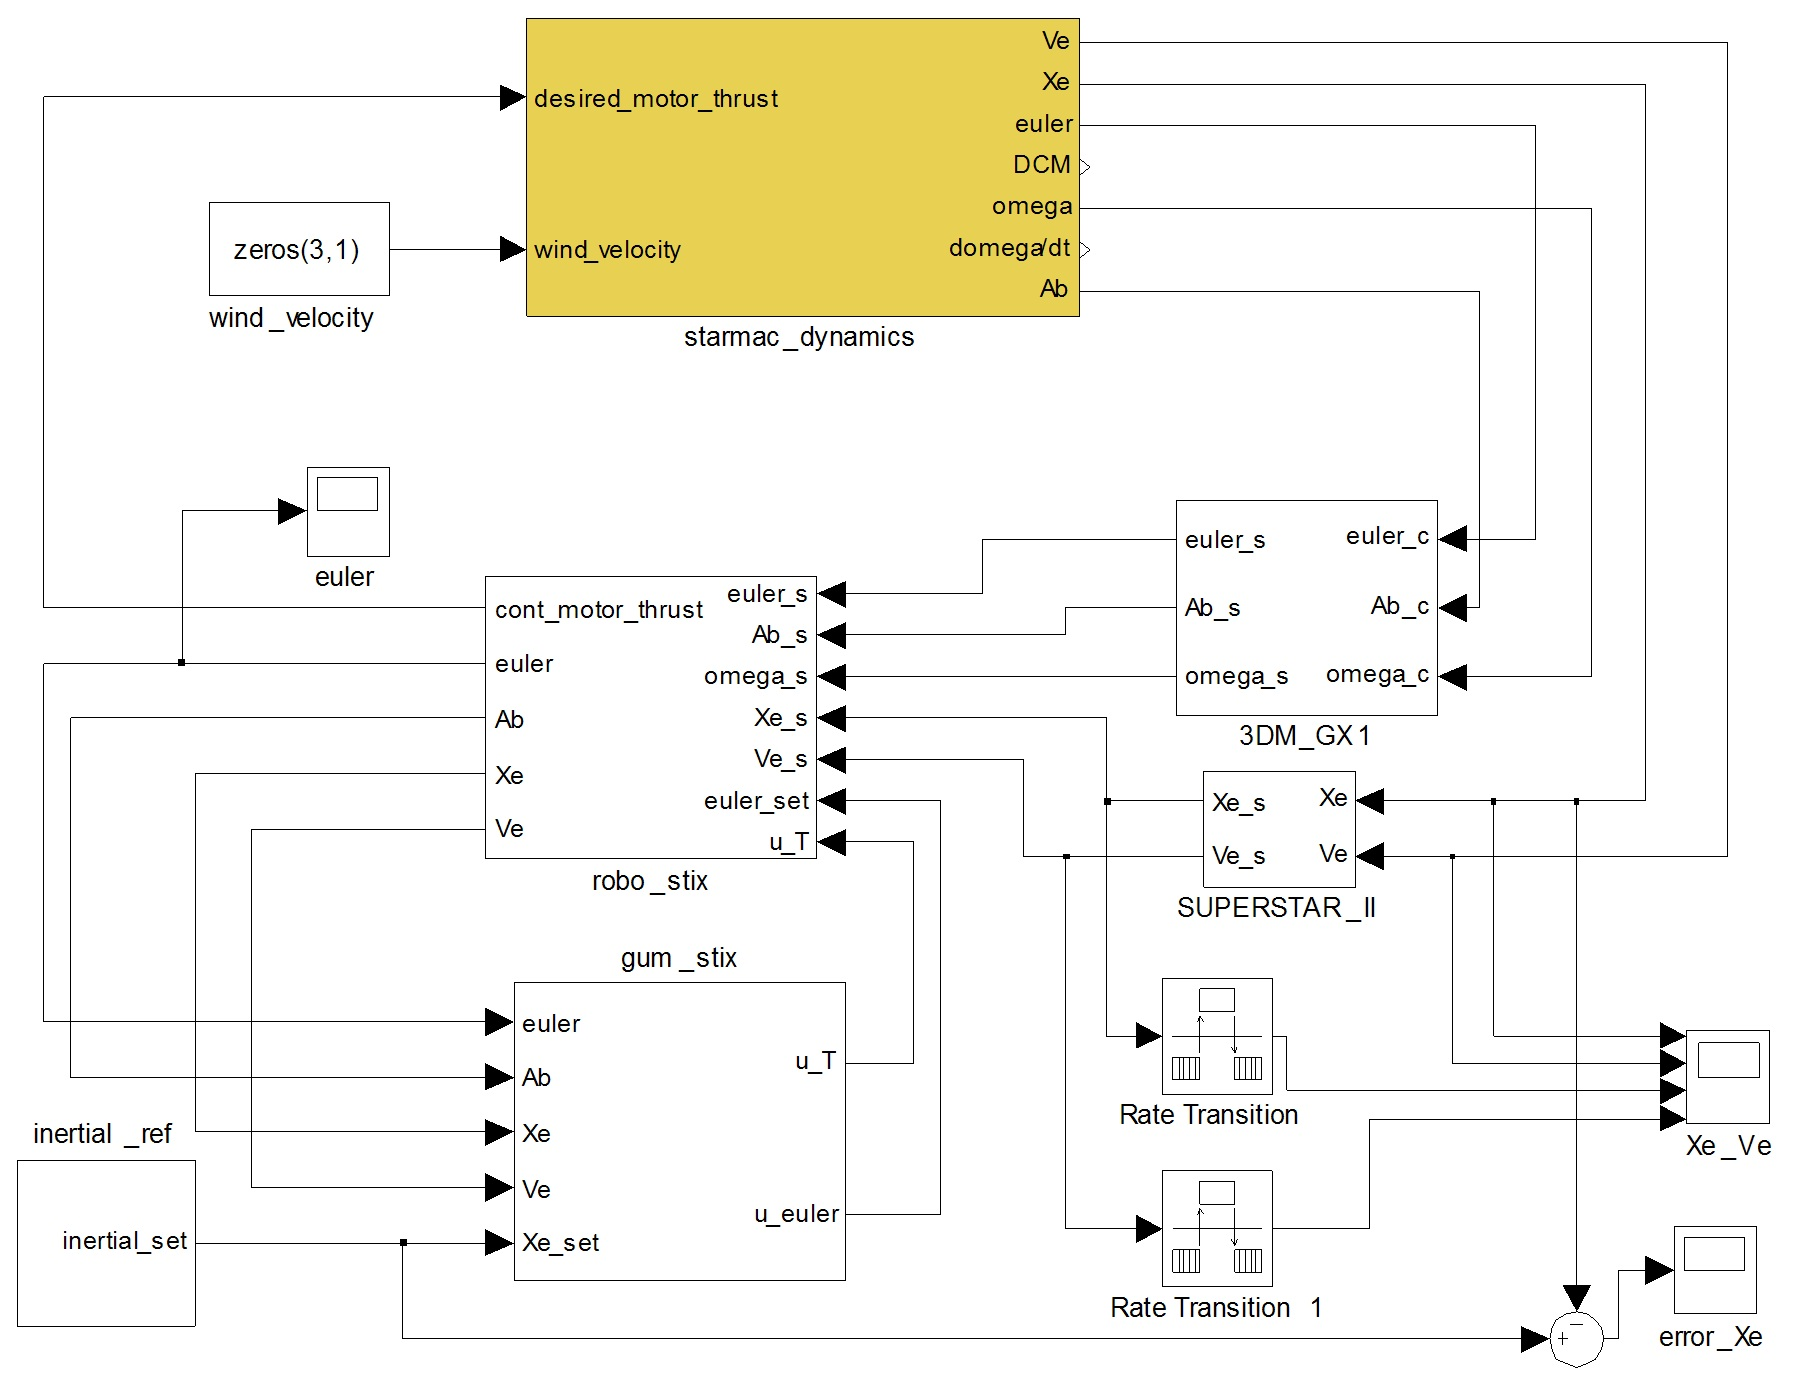
\includegraphics[width=\columnwidth]{figures/starmac_sys.jpg}
%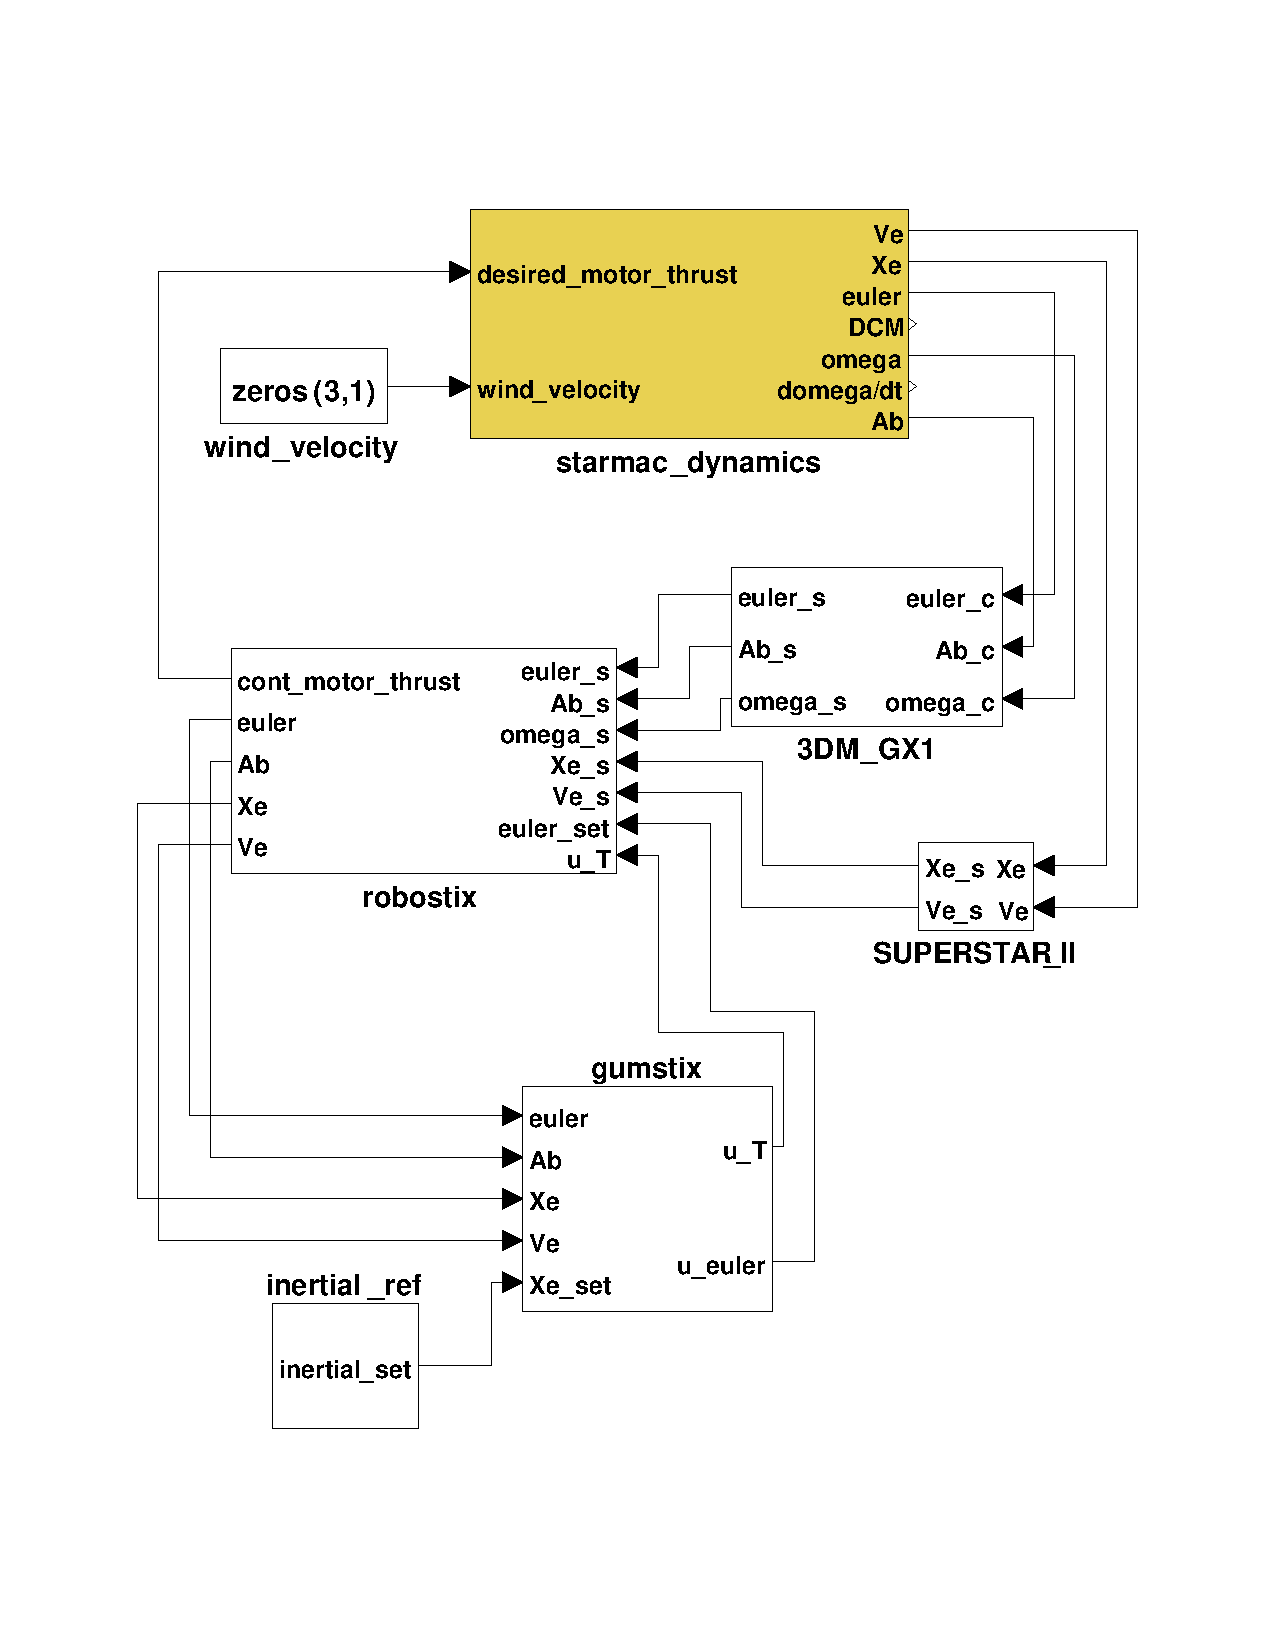
\includegraphics[width=0.9\columnwidth]{figures/starmac_arch_top.pdf}
\includegraphics[width=0.9\columnwidth]{figures/starmac_sys_arch.png}
    \caption{Starmac controller model in Simulink. The dynamics model captures the continuous-time behavior, the IMU (3DM\_GX1) and GPS (SUPERSTAR\_II) blocks model sensors, and the gum\_stix/robo\_stix models contain controller details.}
    \label{fig:starmac}
\end{figure}

A running example in the paper illustrates the use of the toolchain. Fig. \ref{fig:starmac} shows a Simulink model for the Starmac quadrotor helicopter ~\cite{HHWT07}.  The helicopter has a very flexible design for testing onboard computing hardware and sensor options.  One configuration divides computation between a fast, simple inner attitude control loop running on an embedded microcontroller and a slower, more computationally intensive inertial control loop running on a higher-end CPU.  We will describe the model-based development of the respective control software for this configuration.  Distribution over only two processors and a single data bus represents a very simple sample, but one which lends itself to a clear and detailed presentation.  Our results are still preliminary, but we will discuss some of the design problems exposed by the prototype.  We will also cover some related modeling and tool integration efforts.
